

Presentaremos la arquitectura explicando cómo se brindan las funcionalidades requeridas, mencionando diseños alternativos y algunos aspectos relevantes de la comunicación. Por último se comentará cómo se logra cada atributo de calidad a partir de las tácticas utilizadas y la estructura descripta. 

\section{Presentación de la arquitectura}

El uso más habitual que se le dará al sistema será el de votar, por lo que comenzaremos explicando cómo se logra esta funcionalidad con la arquitectura propuesta, enfocándonos principalmente en el diagrama de componentes y conectores.

\begin{figure}[H]
	\begin{center}
		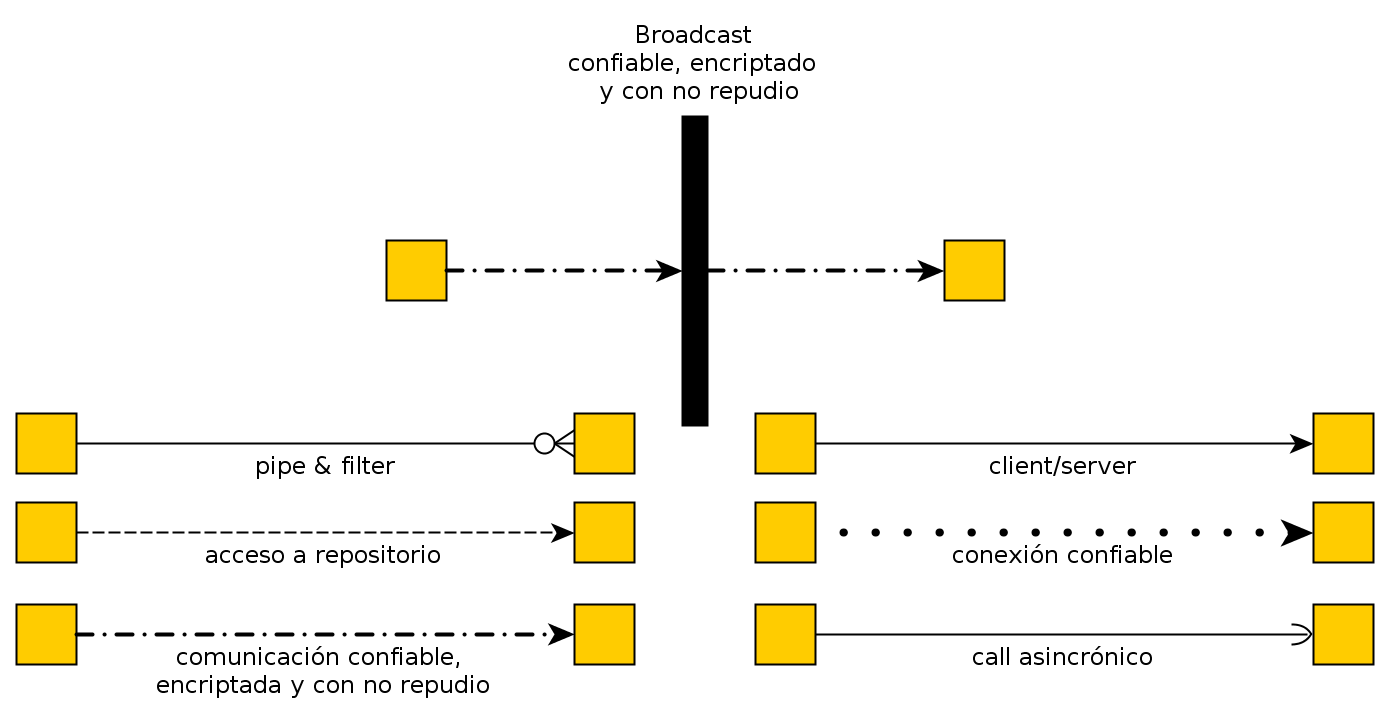
\includegraphics[scale=0.22]{../diagramas/tiposConector.png}
	\end{center} 
	\caption{Conectores utilizados en la arquitectura}
	\label{fig:tiposConector}
\end{figure}

\begin{figure}[H]
	\begin{center}
		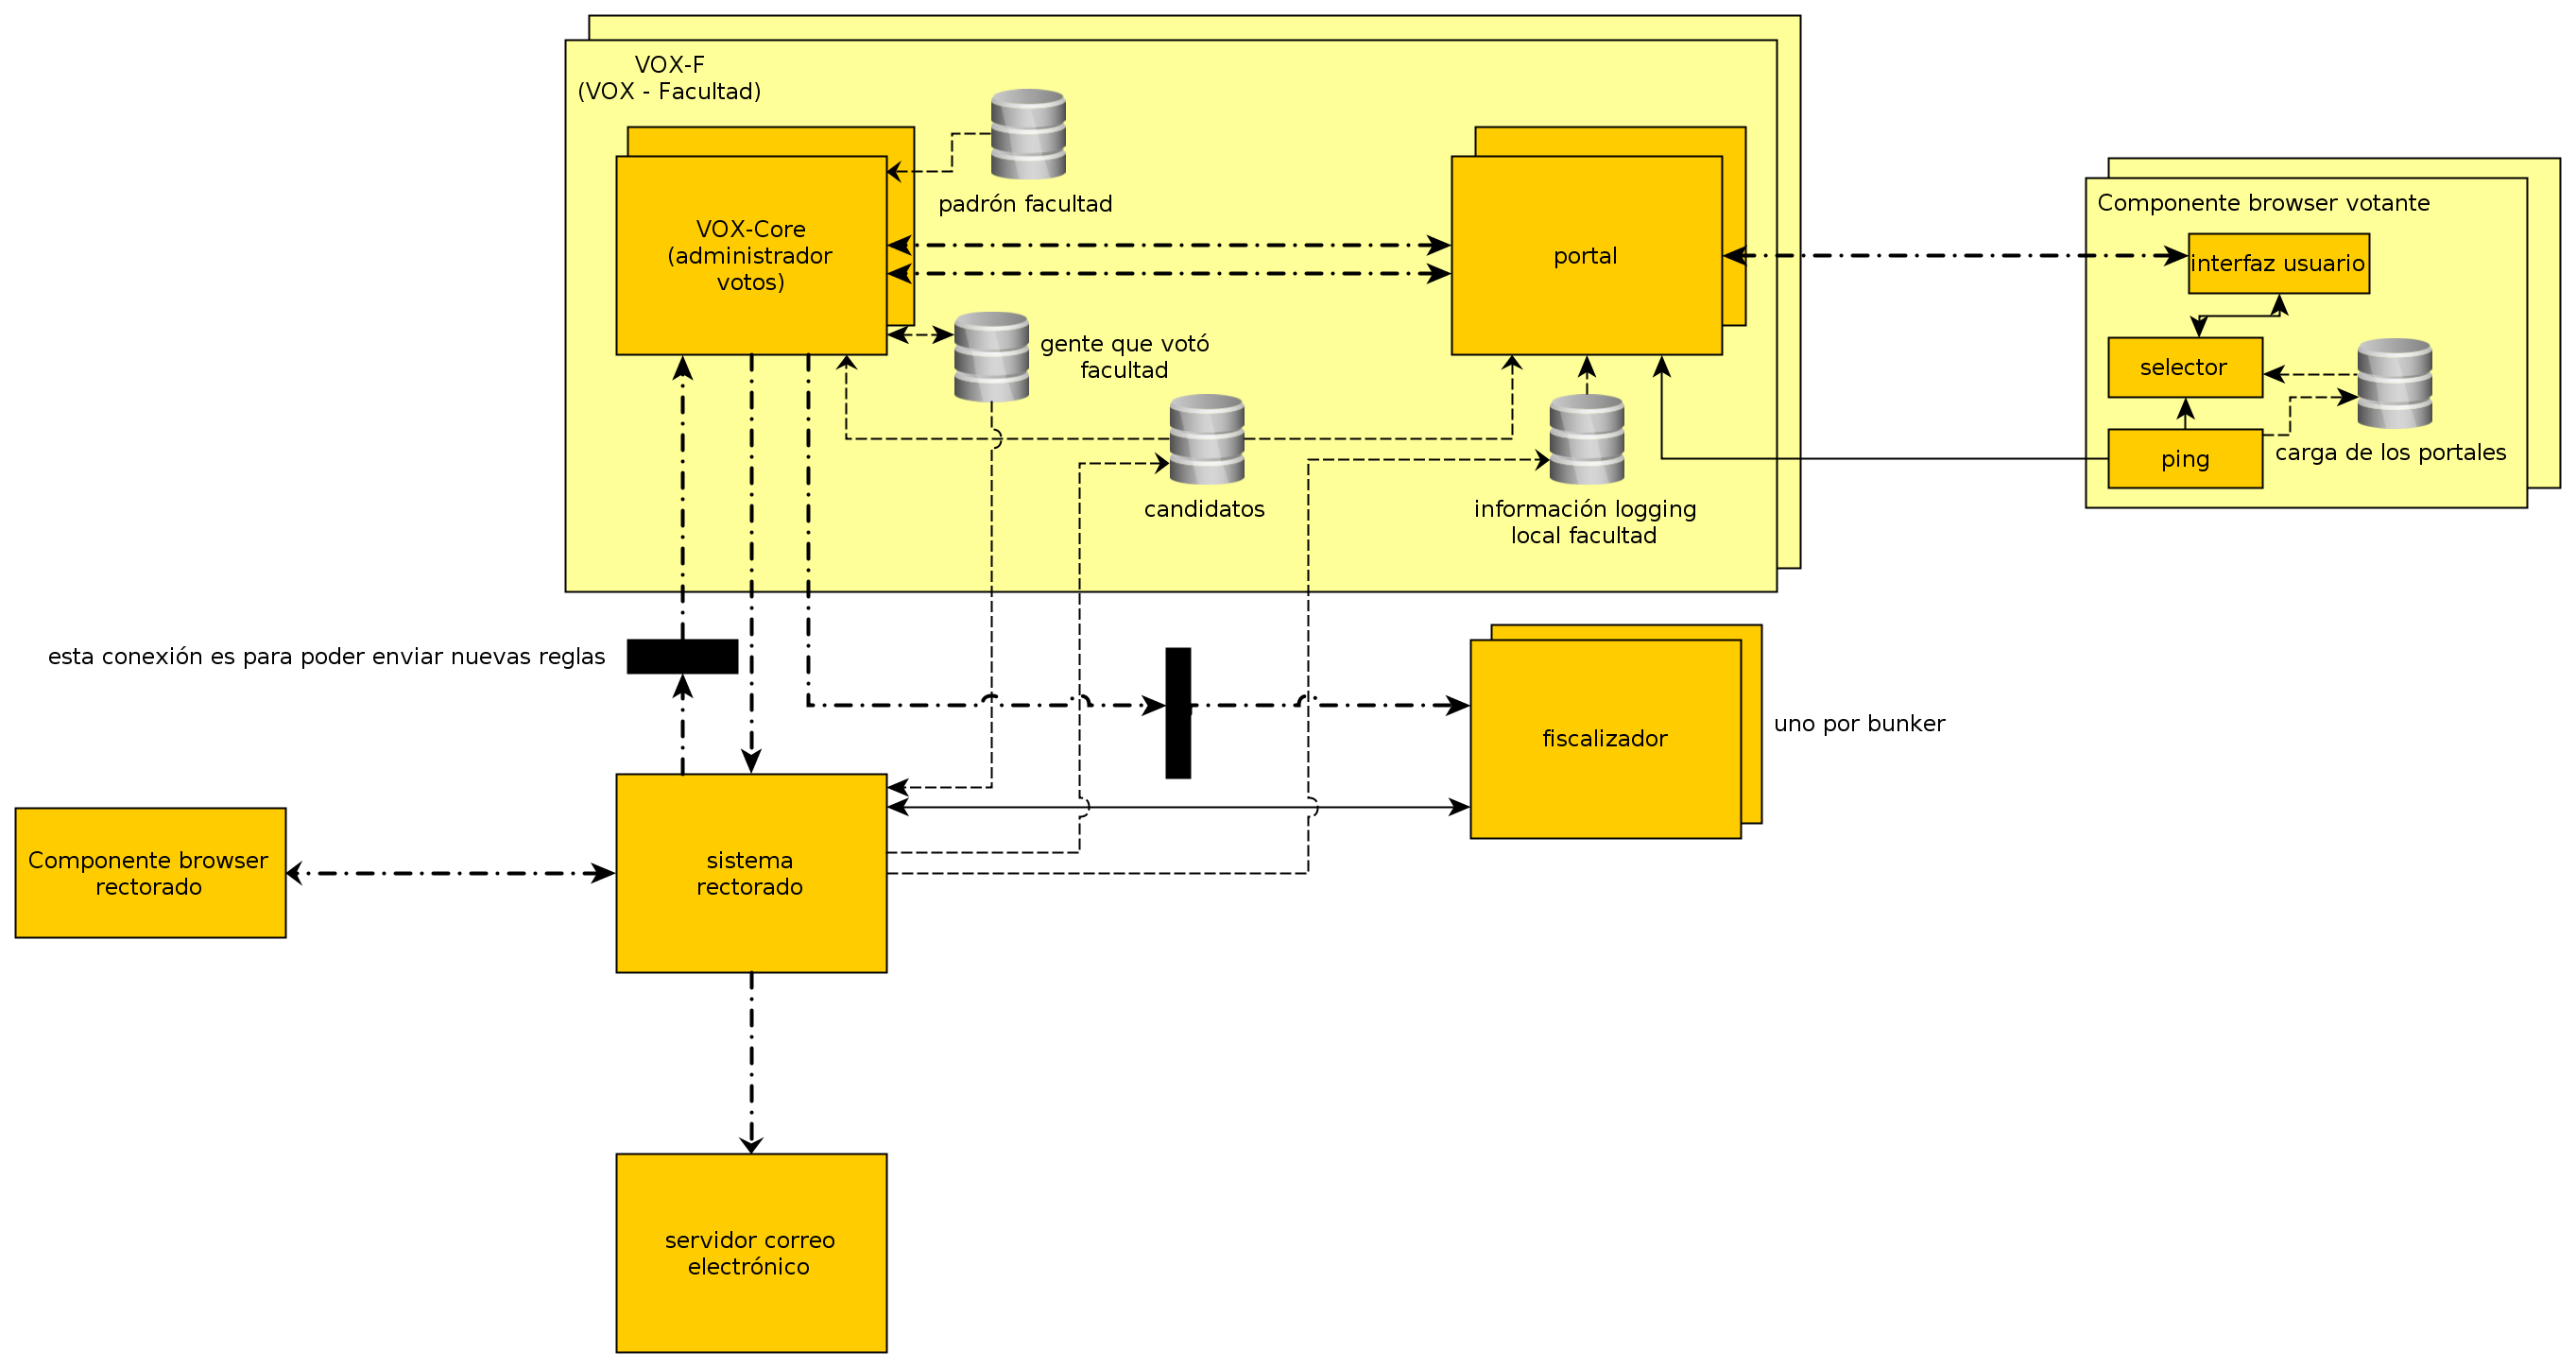
\includegraphics[scale=0.18]{../diagramas/vistaPrincipal.png}
	\end{center} 
	\caption{Componentes y conectores involucrados en la votación}	
	\label{fig:vistaPrincipal}
\end{figure}

Para votar, un usuario deberá conectarse por Internet al sitio designado por su Facultad a tal efecto. El browser que utiliza el usuario se comunicará con el componente Vox de la Facultad. El browser mostrará la opción de autenticarse frente al sistema mediante un nombre de usuario y contraseña, previamente generada por el sistema.

Esta información será enviada por una conexión encriptada y confiable al componente Vox de la Facultad que validará dicha información y retornará al browser un certificado de autenticación que será utilizado subsecuentemente para garantizar que la comunicación cumpla con las características de seguridad deseadas.

Tras autenticar exitosamente al usuario, el browser mostrará los candidatos disponibles, también recibidos del componente Vox de la Facultad. Si el usuario concretara su voto luego recibiría un certificado del mismo, generado por el componente Vox de la Facultad.

Con esta breve introducción se aprecia que será responsabilidad del componente Vox de la Facultad recibir combinaciones de nombres de usuario y contraseña y poder verificar su validez, también contará con la información de los candidatos y por último la capacidad de generar certificados de los votos recibidos, funcionalidades que veremos a continuación.


El componente Vox de la Facultad resultó polémico debido a que gran parte de la funcionalidad será brindada por el mismo y existen varios intereses que entran en conflicto al momento de elegir una arquitectura en particular. Una primera propuesta, que puede verse en la figura \ref{fig:arquitecturaInsegura}
, se apoya fuertemente en la premisa de que los subcomponentes de administración de votos (VOX-Core) y portal online se ejecutarían en servidores diferentes y que podrían existir problemas de conexión entre los mismos, para lo que sería necesario proveer algún mecanismo que permitiera ejercer el derecho a voto aún sin poder contar con las funcionalidades de administración de votos. Esta alternativa no terminó de detallarse porque resultaron evidentes varias complicaciones que ponían en riesgo la seguridad del sistema y algunos criterios de usabilidad. Concretamente los defectos que encontramos en esta opción se relacionan con la necesidad de guardar los votos asociados a sus votantes en un repositorio externo a la facultad hasta tanto se recupere la conectividad con la facultad y que durante ese tiempo de desconexión el usuario no contaría con un certificado de su voto y, en el mejor de los casos, recibiría un mensaje informándole de los problemas de conexión y dejándolo con gran incertidumbre respecto del efectivo cómputo del mismo.


\begin{figure}[H]
	\begin{center}
		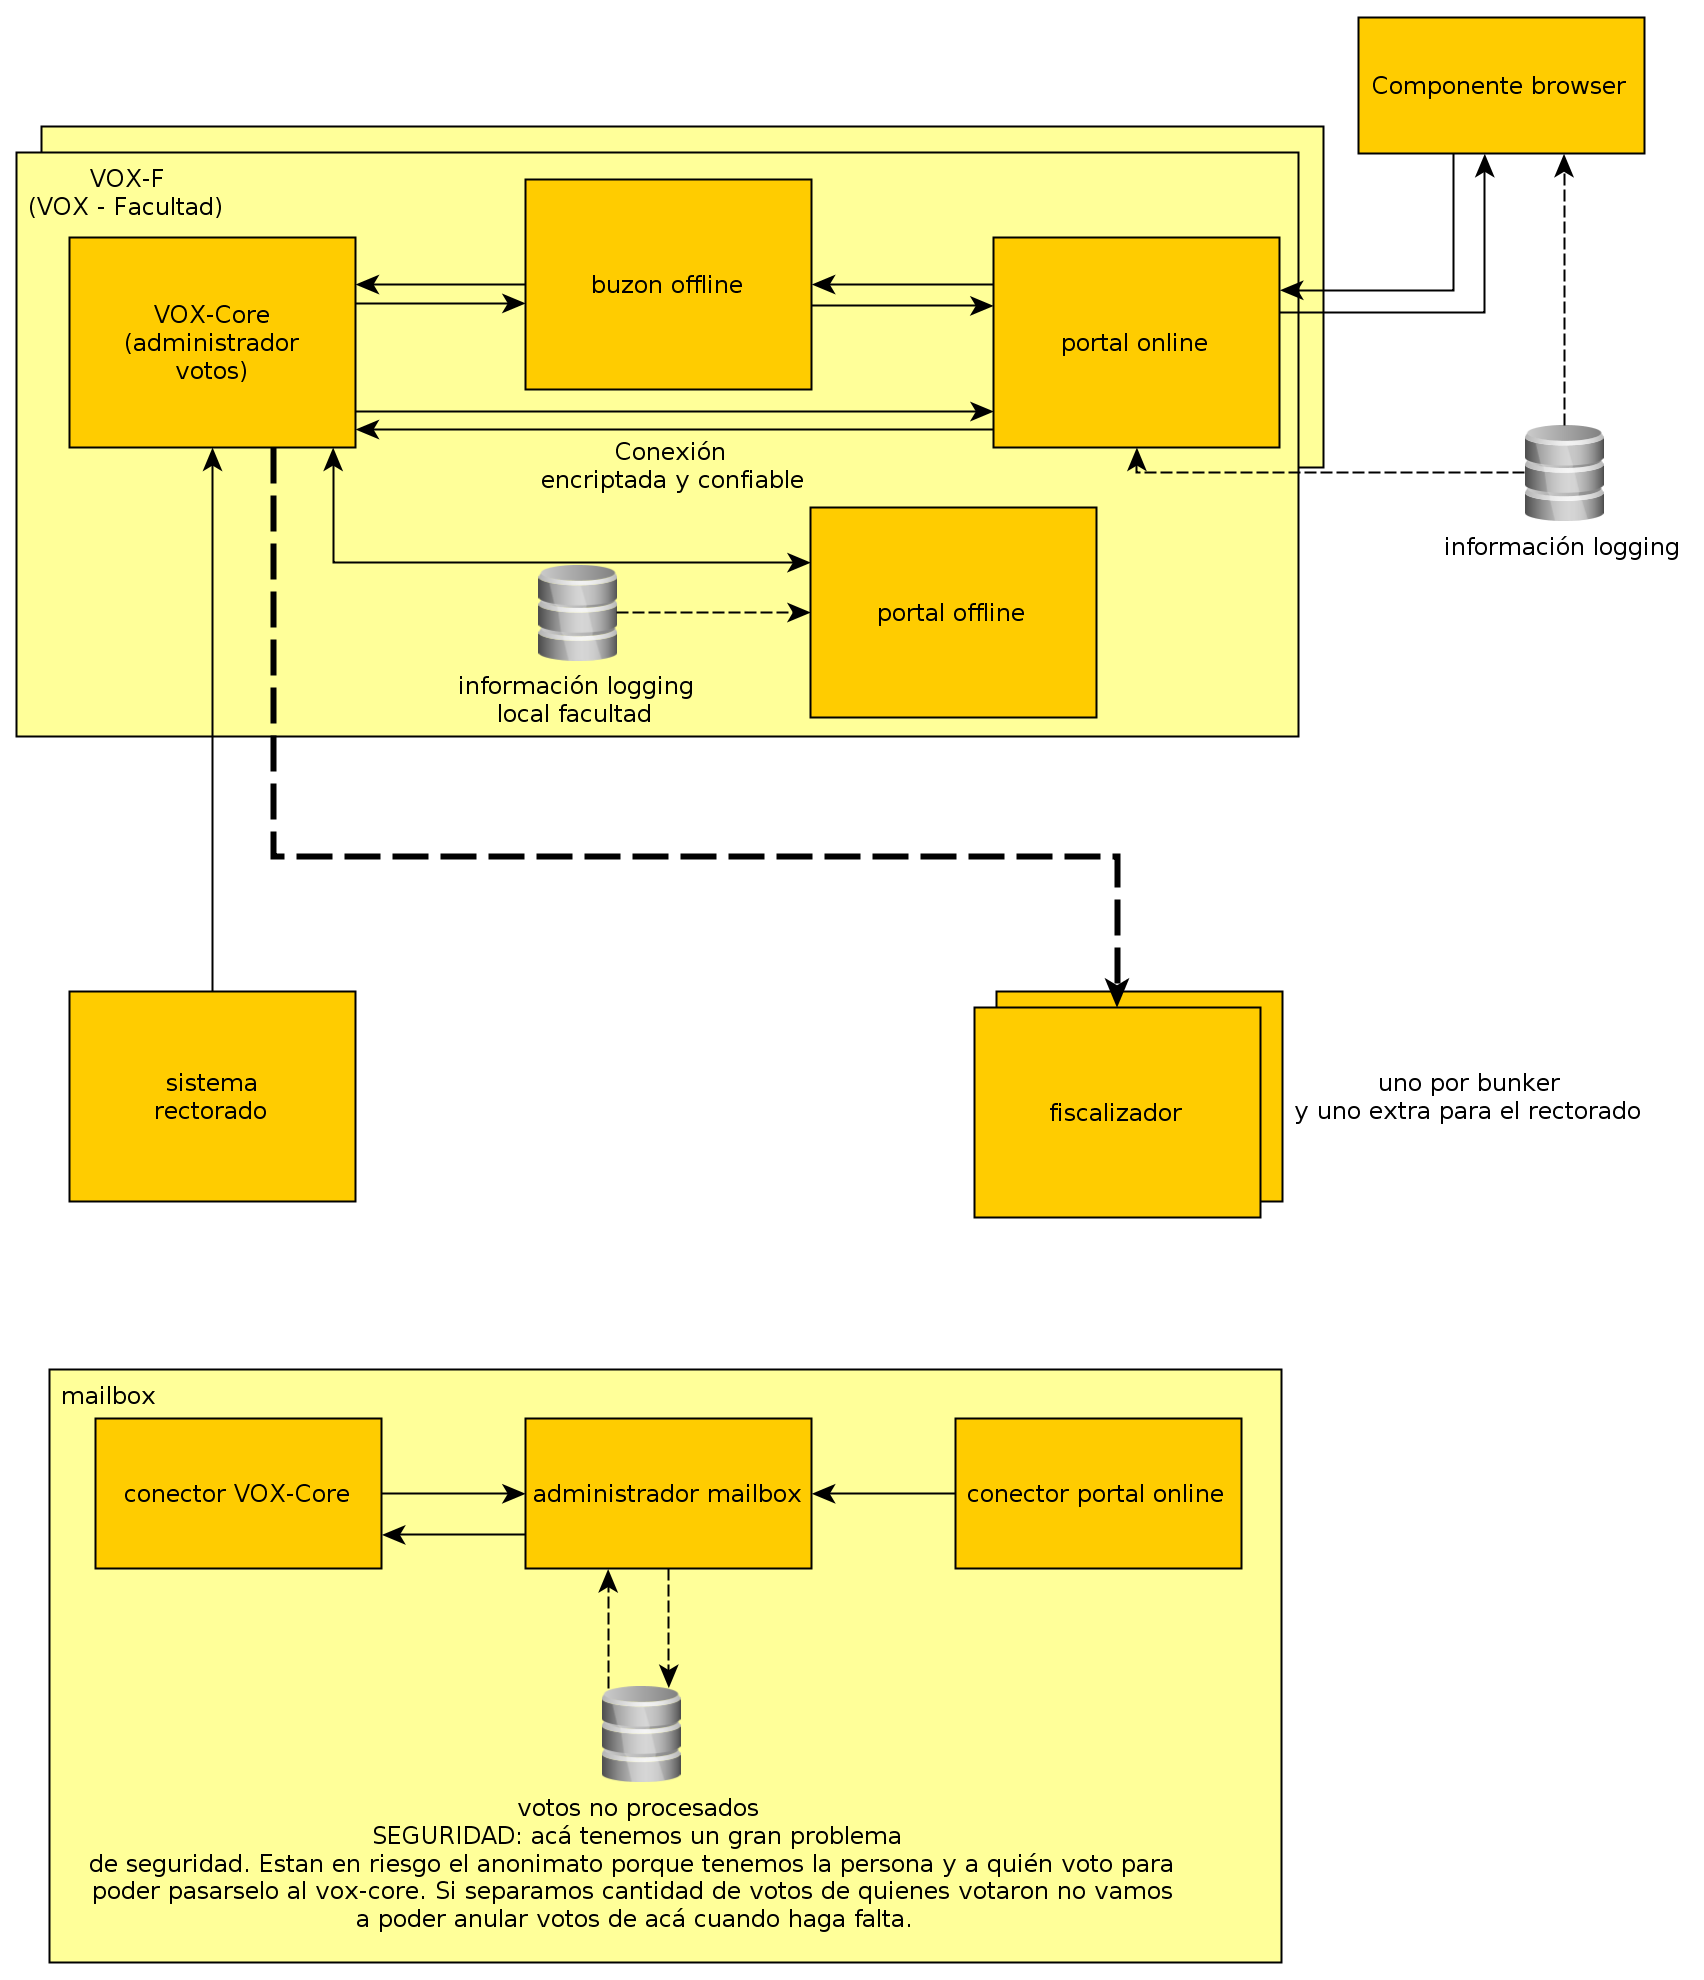
\includegraphics[scale=0.26]{../diagramas/arquitecturaInsegura.png}
	\end{center}
	\caption{Componentes y conectores de la arquitectura que se descarto por insegura}	
	\label{fig:arquitecturaInsegura}
\end{figure}

Considerando la prioridad asignada a los atributos de calidad en el QAW realizado y siendo confiabilidad menos prioritario que usabilidad y que seguridad optamos por favorecer una estructura diferente, que aporta menos garantías de confiabilidad pero mejora sensiblemente los aspectos antes mencionados de usabilidad y seguridad.

Se puede apreciar en la figura \ref{fig:vistaPrincipal} % TODO referenciar al diagrama
que en la propuesta elegida se elimina la necesidad de mantener un repositorio de votos no procesados, como ocurría con la anterior opción. Sin embargo, para poder mantener la posibilidad de votar en todo momento, será necesario que alguna de las instancias del portal esté siendo ejecutado en la Facultad misma. 

La estructura propuesta permite que el conteo de votos se lleve a cabo en cada Facultad independientemente de las demás, pero esta descentralización, junto con la necesidad de fiscalizar los resultados realizando un recuento completo, conlleva un costo elevado en cuanto a la complejidad de la conexión entre las distintas facultades y los componentes correspondientes a la fiscalización realizada por cada agrupación política y por el rectorado.

Para apreciar el funcionamiento del componente Vox-Facultad, ver figura \ref{fig:voxcore}, seguiremos los pasos a realizarse para el proceso de un voto, asumiendo que la autenticación ya fue realizada. Una vez arribado el voto, a través del componente portal, el mismo es transmitido dentro de un mensaje al administrador de votos, junto con el nombre de usuario del sufragante. Dentro de VOX-Core, el componente del comunicador desencripta el mensaje y lo envía al chequeador de reglas, que consulta el repositorio padrón(donde se encuentra toda la información pertinente de los alumnos) y verifica el cumplimiento por parte del usuario de las restricciones impuestas por rectorado.

El curso del mensaje continúa por el chequeador de candidatos, que verifica la validez del candidato accediendo al repositorio de candidatos.
Luego el mensaje avanza al chequeador de votos repetidos que, mediante un acceso al repositorio de gente que votó, verifica que el usuario no haya votado.
Por último, y de haberse superado con éxito todos los chequeos impuestos por los filtros, el componente auditor registra un voto para el candidato correspondiente, se envía el voto al publicador y se genera, a partir del sistema externo HardToBreak, un certificado de la emisión del voto, que es retornado al comunicador. Es importante destacar que el voto en sí no contiene información del votante, pero podría contener algún tipo de hash o certificado, que mejore la auditabilidad del sistema. 
 
\begin{figure}[H]
	\begin{center}
		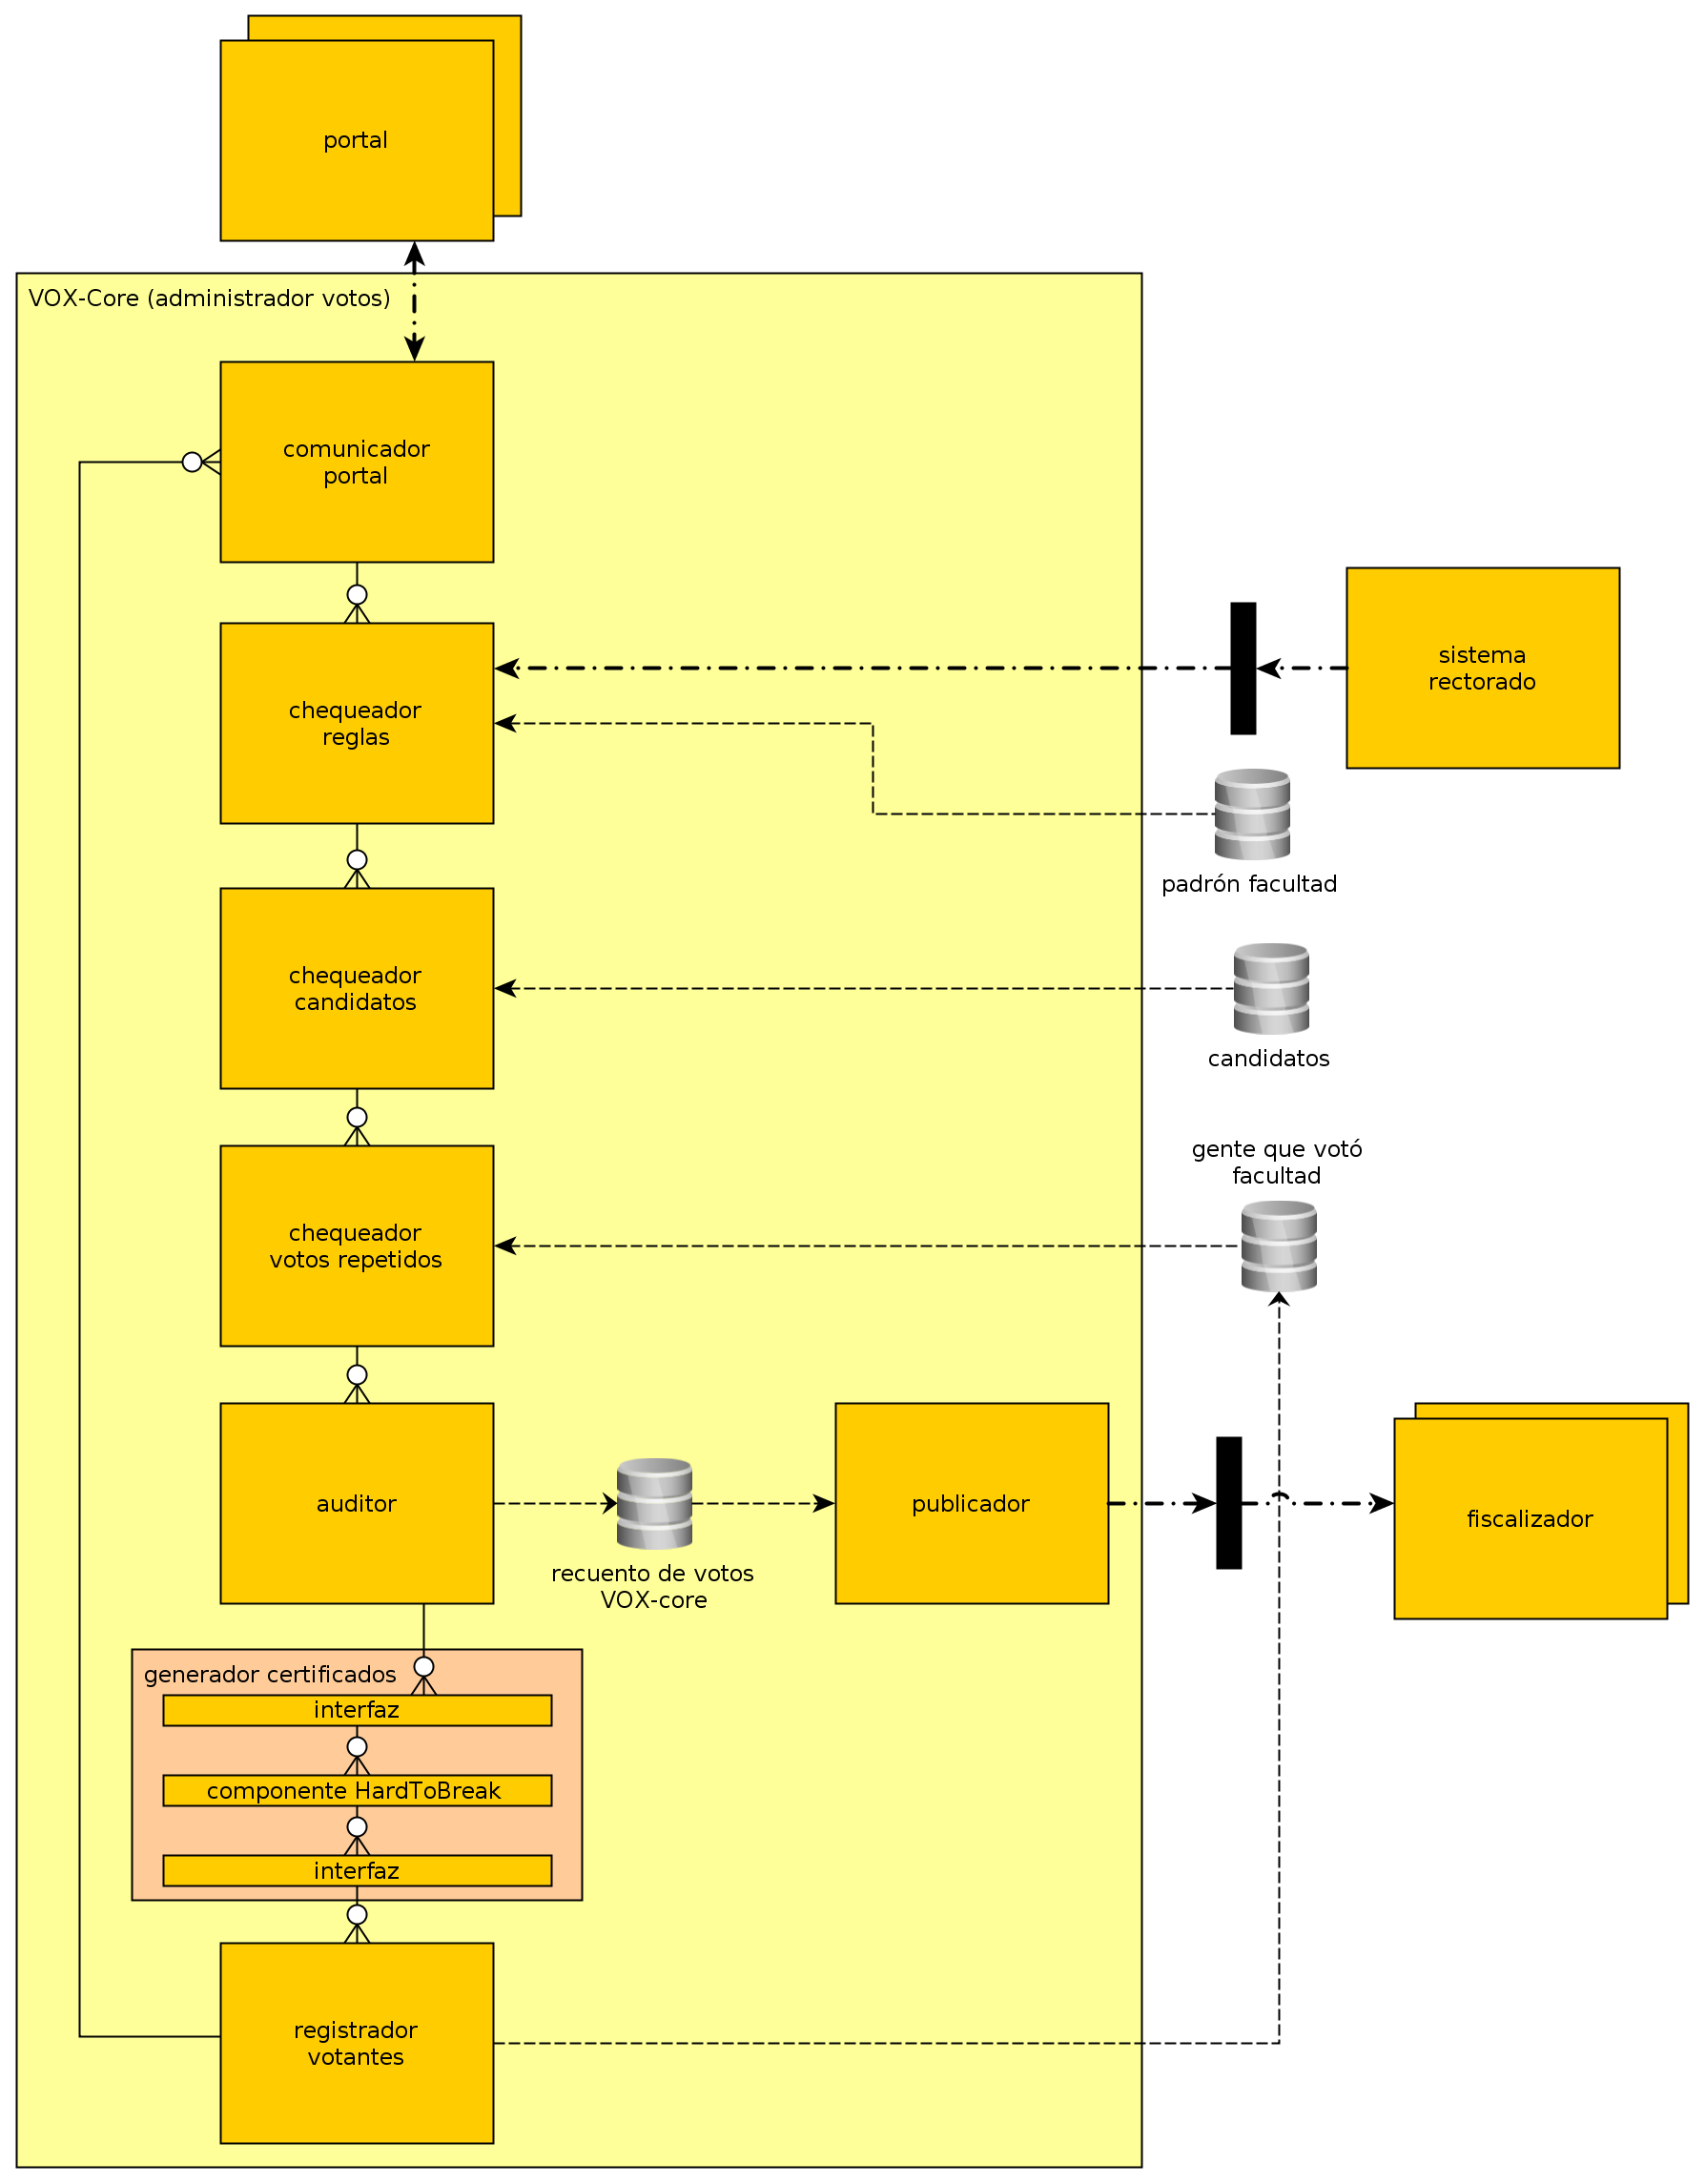
\includegraphics[scale=0.26]{../diagramas/voxcore.png}
	\end{center}
	\caption{Vista ampliada del componente VOX-core}	
	\label{fig:voxcore}
\end{figure} 
 
Para satisfacer las necesidades de fiscalización expresadas, tras procesarse el voto, el mismo es recibido por el publicador, 
para luego ser enviado a través de un conector broadcast seguro, confiable y con no-repudio. Si bien podría ser deseable utilizar un esquema similar al de publish and subscribe, es conveniente priorizar la seguridad y sólo permitir el envío de los paquetes a componentes agregados manualmente mediante archivos de configuración, para evitar la posibilidad de que se engañe al sistema y un atacante reciba la información.

El proceso que seguirá una vez recibido por los componentes fiscalizadores de las agrupaciones políticas y rectorado consiste en registrar el voto para el candidato correspondiente. La frecuencia con que efectivamente se envían los votos deberá determinarse con mayor participación de los diferentes stakeholders, ya que el envío inmediato de los votos junto con la posibilidad de acceso en todo momento a la información de los votantes que ya emitieron su voto hace imposible la tarea de mantener el voto secreto. El funcionamiento de la cola de envíos implementada en el publicador queda por el momento indefinido, pero puede ser tan simple como enviar inmediatamente los votos encolados hasta un esquema más complejo, que contenga restricciones sobre la mínima cantidad de votos acumulados o la mínima cantidad de candidatos representados en los mismos, por ejemplo.

%%felipe-----------------
En cada componente fiscalizador,  ver figura \ref{fig:fiscalizador}, se recibe el conteo de votos de todas las facultades y se calculan los resultados totales. Luego mediante la interfaz por browser del fiscalizador es posible filtrar qué porcentajes se muestran.

\begin{figure}[H]
	\begin{center}
		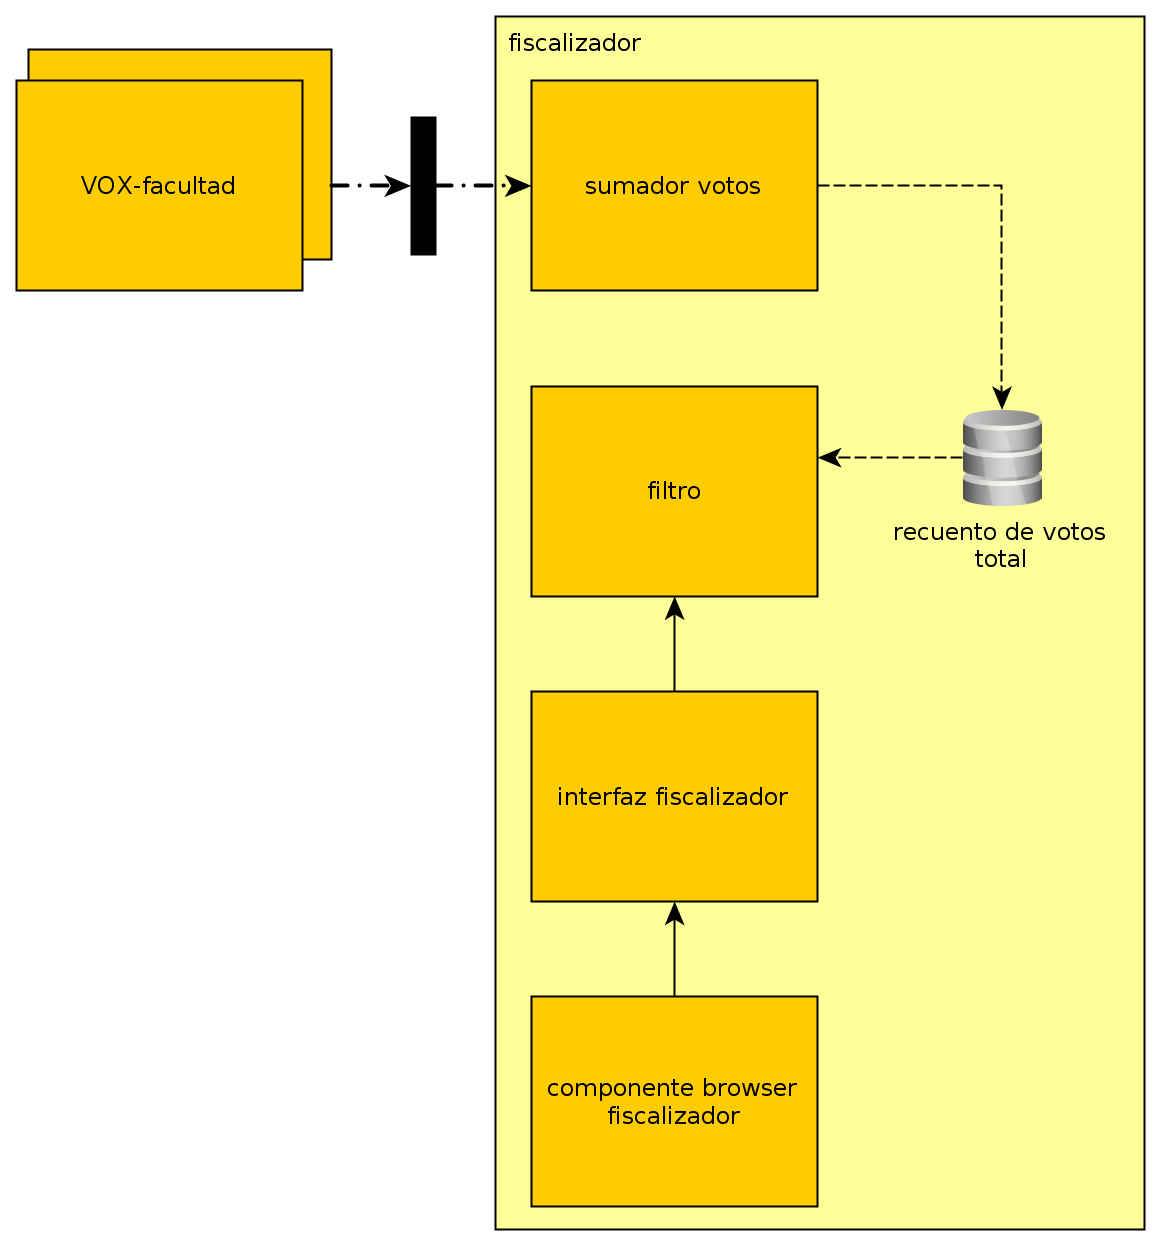
\includegraphics[scale=0.26]{../diagramas/fiscalizador.png}
	\end{center} 
	\caption{Vista ampliada del componente fiscalizador}	
	\label{fig:fiscalizador}
\end{figure} 

El componente dedicado a las tareas administrativas del rectorado permite, ver figura \ref{fig:sistemaRectorado}, mediante una cómoda interfaz por browser, administrar las reglas de los comicios y enviarlas por broadcast a todas las facultades. La interfaz también da un marco para ingresar los candidatos que luego se propagarán a los repositorios de los componentes Vox-Facultad. También da la opción de generar el acta de los comicios, comunicándose con su fiscalizador para obtener los resultados totales.
\\
Desde el sistema de rectorado se generan, antes de iniciar los comicios, las contraseñas para todos los usuarios y se les envía al correo electrónico que tengan registrado en el padrón. Luego a cada facultad se le envía la información necesaria para registrar el loggueo de sus votantes.
\\
\\
En el diagrama se realizó una abstracción para facilitar la comprensión del funcionamiento de este componente. Donde el sistema del rectorado accede a los repositorios de los componentes VOX-facultad, en el diagrama se lo indica con un acceso a repositorio de un modulo a otro, aunque no se indica que el acceso se realiza a travez de VOX-facultad usando la conexión segura, confiable y con no-repudio que comunica el componente del rectorado con los VOX-facultad.
%%felipe-----------------

\begin{figure}[H]
	\begin{center}
		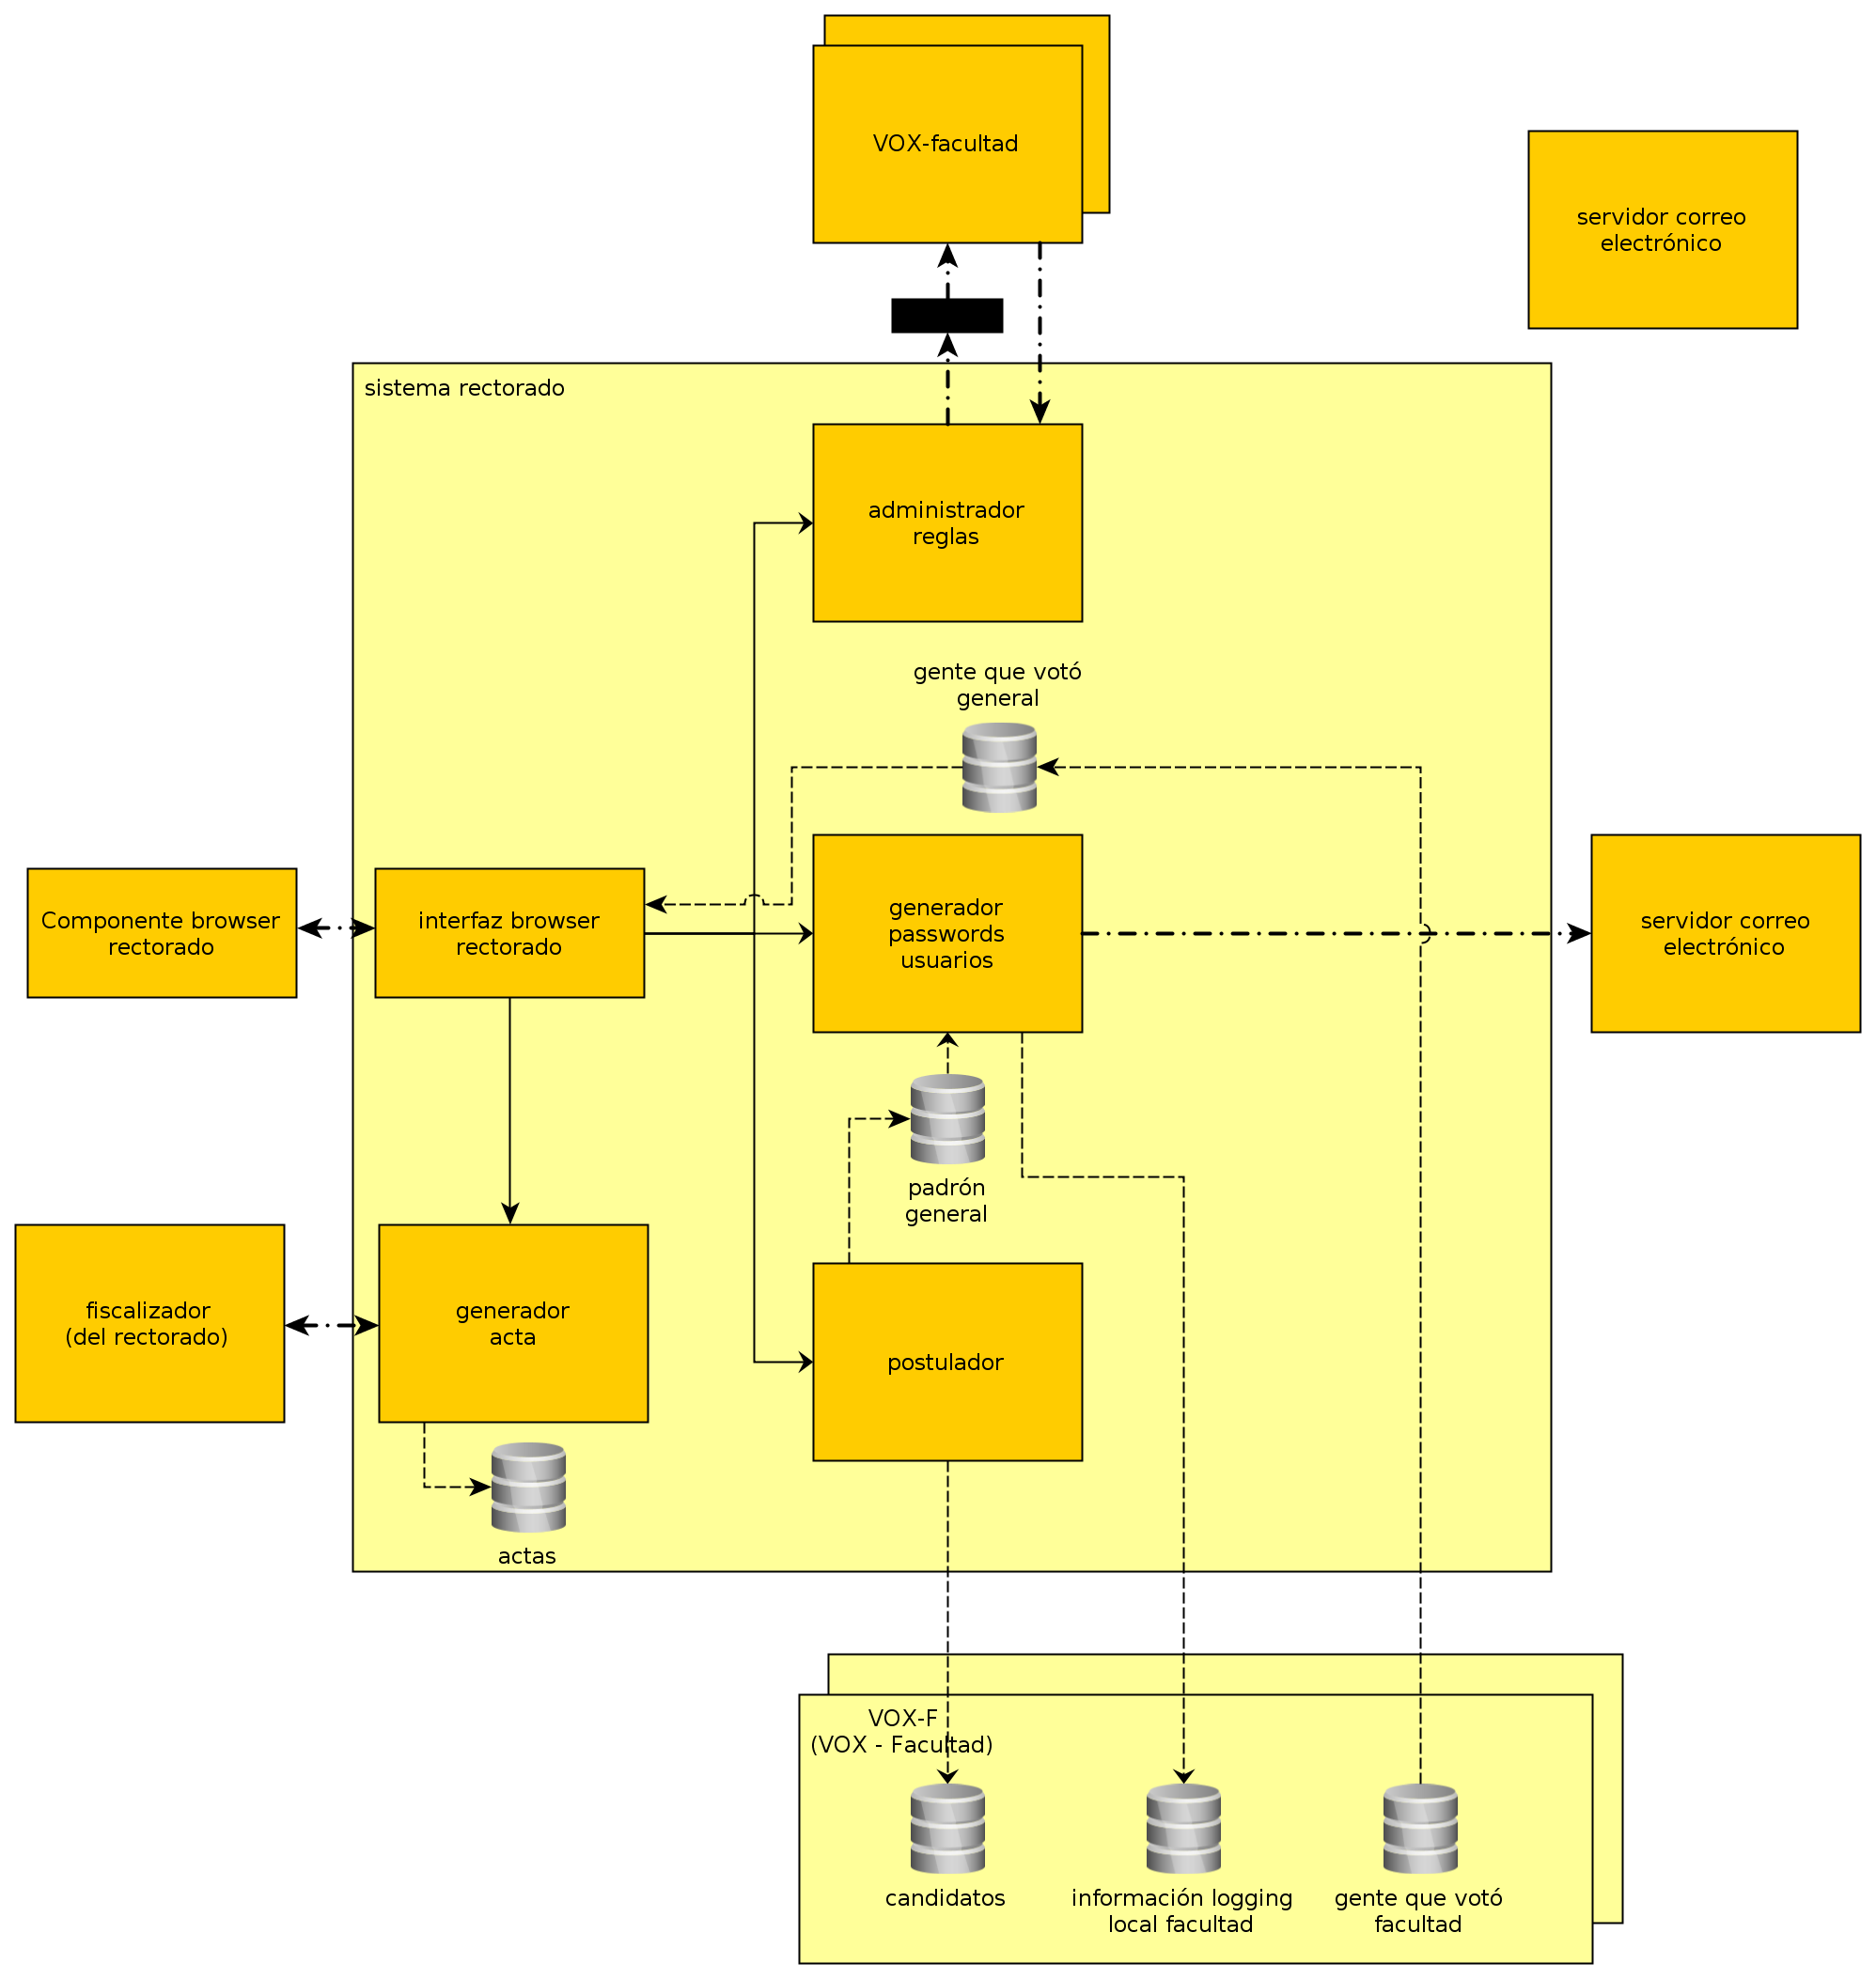
\includegraphics[scale=0.26]{../diagramas/sistemaRectorado.png}
	\end{center}
	\caption{Vista ampliada del componente dedicado al rectorado}
	\label{fig:sistemaRectorado}
\end{figure} 

El comunicador merece una discusión aparte por sus varias particularidades, , ver figura \ref{fig:comunicador}. Recordemos que el comunicador debe ofrecer comunicación encriptada, confiable y no repudiable. Dado que no repudiación se logra a partir de la utilización de firmas digitales, consideramos esa explicación secundaria y nos centraremos en explicar cómo se logra encriptación y confiabilidad.

Esencialmente la tarea del comunicador, al recibir datos que tiene que enviar, encriptará los datos, generará un mensaje con la información necesaria para que el otro extremo pueda procesar el mensaje, mandarlo y esperar una respuesta del otro extremo confirmando la recepción.
En el caso de la recepción de un mensaje, se realiza el proceso inverso, se procede a desempaquetar los datos, luego se los desencripta y se entrega dichos datos al componente encargado de procesarlos.

En caso de que se detecte un intento de violar la encriptación o falsificar la autenticación dicha información se almacenara en un log de ataques.

Como se puede apreciar, en el caso de la conexión entre el browser y el portal, es necesario utilizar algún tipo de entidad certificante, ya que no se puede determinar la identidad del servidor de otra manera. Esto genera un pequeño cambio en los componentes, ya que el componente de encripción deberá comunicarse con la entidad certificante para obtener la clave pública del portal.

\begin{figure}[H]
	\begin{center}
		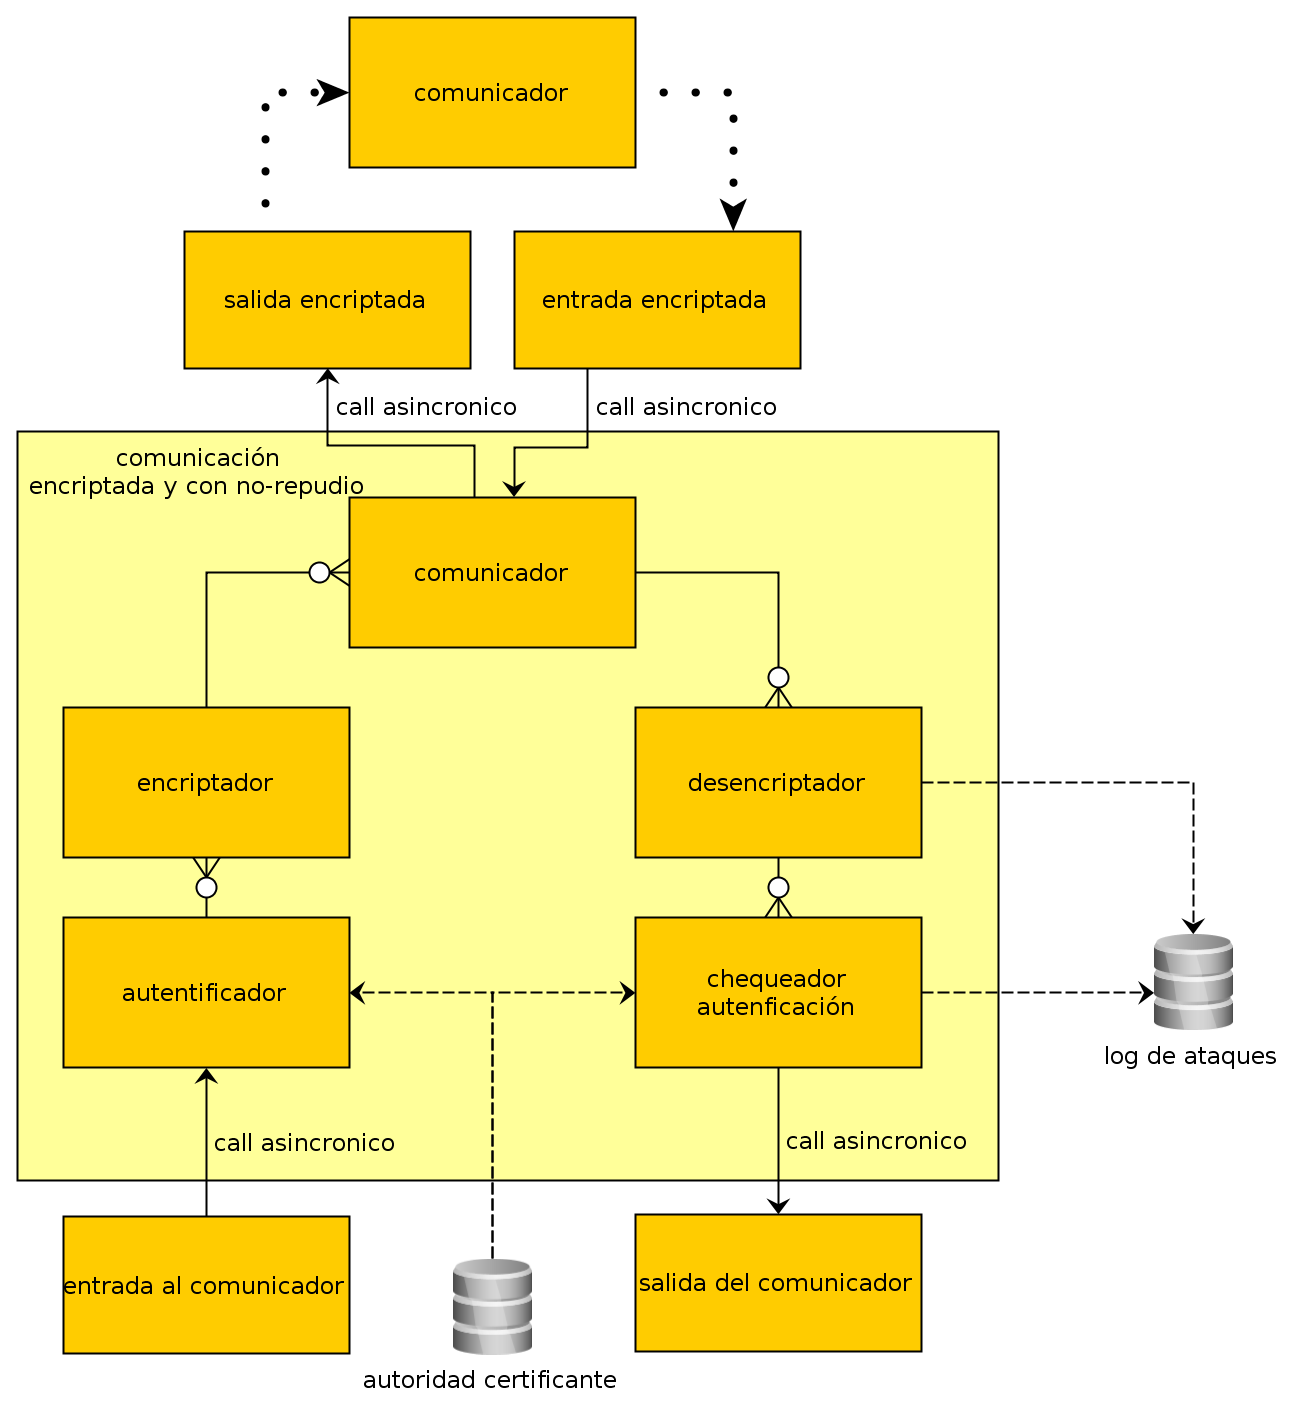
\includegraphics[scale=0.26]{../diagramas/conector.png}
	\end{center} 
	\caption{Vista ampliada del componente dedicado al conector desarrollado}	
	\label{fig:comunicador}
\end{figure} 

% TODO seguir explicando 
\paragraph{Formato de los paquetes} Los paquetes que van de la interfaz de usuario al portal son del tipo usuario-voto. Si bien en este punto está presente un riesgo de seguridad la encriptación protege el anonimato del votante. Cuando la interfaz se comunica con VOX-core empaqueta el mensaje del votante en un nuevo paquete con la información del portal. De esta manera el componente VOX-core tiene suficiente información para registrar el voto, registrar que el emisor del mismo ya votó y además devolverle un certificado.

\subsection{Estilos y Tácticas}

Al crear la arquitectura, nos ayudamos fuertemente en las tácticas que nos provee la bibliografía para atacar los distintos atributos de calidad relevados. A su vez, analizándola, entendemos que no nos quedamos con un estilo puro, sino que tomamos varios aspectos de distintos estilos, particularmente obtuvimos cierta inspiración en \textit{Pipe and Filters, Call Returns y Client-Server}. \\ A continuación presentamos los aspectos relevados, organizados en la taxonomía propuesta por la bibliografía para los atributos de calidad, y cómo impactaron en nuestra arquitectura.
 

\paragraph{Seguridad}
Dada la necesidad de asegurar un nivel elevado de seguridad en todos los niveles, se utilizaron varias tácticas con dicho objetivo. En todas las comunicaciones se utiliza encriptación, suma de verificación y un esquema de firmas certificadas para garantizar no repudio. La conexión de las interfaces gráficas para los votantes con el resto del sistema utilizan autenticación. Además se incorpora un log de ataques para llevar cuenta de los intentos de vulnerar las comunicaciones del sistema. De esta manera logramos trazar la arquitectura con varias de las tácticas de seguridad sugeridas por la bibliografía.

\paragraph{Usabilidad}
Para mejorar la usabilidad se separó la interfaz gráfica del resto de los componentes, de manera que pueda mutar por separado, priorizando criterios de facilidad de uso y de aprendizaje, tal como suguiera la táctica \textit{Separece User Interface}. A su vez, la interfaz de usuario presenta la necesidad de confirmar el voto. Además se puede utilizar diferentes interfaces cambiando de componente browser. De esta manera es posible usar el sistema en diferentes plataformas tecnológicas (tablets, smartphones, etc) y desarrollar nuevas interfaces para usuarios con capacidades diferentes.

\paragraph{Performance/Disponibilidad}
El portal,  ver figura \ref{fig:portal}, elige con qué componente VOX-core se va a comunicar para distribuir la carga entrante y permitir una mejor respuesta del sistema, siguiendo la táctica \textit{Scheduling Policy}. Mediante \textit{Ping/Echo} logramos censar la disponibilidad de cada Vox-Core que se quiere conectar. En horas pico se puede activar un mayor número de componentes VOX-core para lidiar con el flujo de usuarios siguiendo la táctica de \textit{Increase Available Resources}. La misma estrategia se aplica entre el componente browser y el portal de VOX-facultad.
Todos los repositorios admiten accesos concurrentes, recurriendo a la táctica \textit{Introduce Concurrency}.
\begin{figure}[H]
	\begin{center}
		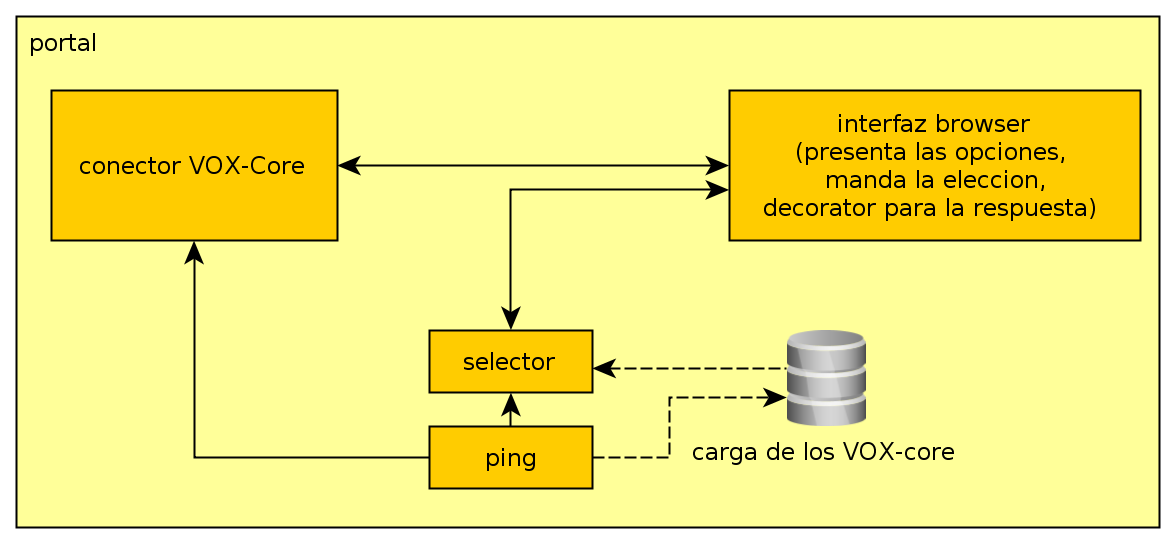
\includegraphics[scale=0.22]{../diagramas/portal.png}
	\end{center}
	\caption{Componente portal ampliado}	
	\label{fig:portal}
\end{figure}

\paragraph{Disponibilidad}
Los repositorios que deberían ser accedidos por todos los componentes VOX-core se replican en cada componente VOX-facultad para disminuir el volumén de consultas, aprovechando la redundancia, indicado bajo el nombre \textit{Redundancy}.

\paragraph{Modificabilidad}
Dentro del componente VOX-core la funcionalidad que genera el certificado de voto para el usuario está aislada en un componente que define una interfaz para el componente externo. De esta manera si se decide cambiar el sistema que genera los certificados, las modificaciones se acotarán a cambiar sólo ese componente y su interfaz, bajando el impacto gracias al anticipo del posible cambio, siguiendo esta vez las directivas de \textit{Anticipate Expected Changes}. En el caso que el Rectorado decida cambiar las reglas para las elecciones, éste podría hacerlo configurandolas en tiempo de ejecución, inspirado en \textit{Configuration Files}.


